%!TEX root = principal.tex
\chapter{Gerenciamento da manufatura: PIMS e MES}

 PIMS -- \emph{Process Information Management System} e MES -- \emph{Manufacturing Execution System} são sistemas da camada 3 da pirâmide de automação, responsáveis pelo armazenamento e tratamento de dados do nível 2, concentrando os dados de diversos processos separados em um único ponto. São os chamados \emph{middleware}, pois ficam a meio caminho entre os sistemas de gerenciamento de empresa e os supervisórios, às vezes combinando funções de um ou de outro.

 De forma geral, no terceiro nível da pirâmide a preocupação é em consolidar os dados brutos do processo (\emph{data}), para com eles gerar informações  (\emph{information}) e conhecimento (\emph{knowledge}) sobre o processo, aumentando o valor destes valores, como mostra a figura \ref{fig:PIMS_conhecimento1}. Os dados são obtidos ou do controlador ou do supervisório de um determinado processo. A relação entre dados ou a variação destes dados no tempo geram informação sobre a planta. A relação entre informações ou a variação de informações no tempo geram conhecimento.
\begin{figure}[htb]
	\begin{center}
	%	\includegraphics[angle=-90,width=0.8\textwidth]{PIMS_conhecimento1}
		\begin{tikzpicture}[scale=1.5]
		\draw[very thick, ->, >=stealth'](0,0)--(5.5,0);
		\draw(5.5,0)node[below left]{Quantidade de dados};
		\draw[very thick, ->, >=stealth'](0,0)--(0,3.3);
		\draw(0,3.3)node[above left, rotate=90]{Valor};
		\draw[very thick] plot[smooth, tension=1.0] coordinates{(0.2,3.3) (2,1) (5.5,0.3)};
		\draw(0.3,3.)node[right]{Conhecimento} (1.3,1.4)node[above right]{Informação} (4.3,0.4)node[above]{Dados brutos};
	\end{tikzpicture}

	\end{center}
	\caption{Relação entre dados, informações e conhecimentos.}
	\label{fig:PIMS_conhecimento1}
\end{figure}

Um exemplo desta relação é mostrado na figura \ref{fig:PIMS_conhecimento2}. Nesta figura, a partir dos dados de temperatura e vazão de um fluido é gerada a informação do calor removido em determinado trocador de calor. A comparação dos calores removidos de diversos trocadores gera o conhecimento de qual trocador é mais eficiente.

\begin{figure}[htb]
	\begin{center}
		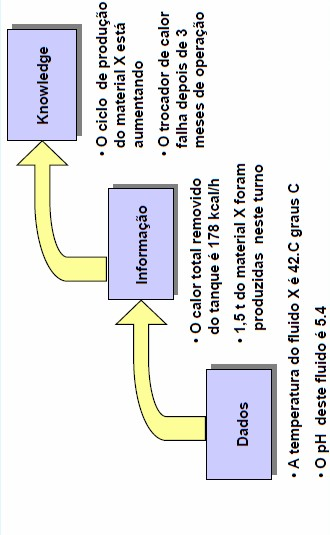
\includegraphics[angle=-90,width=0.8\textwidth]{PIMS_conhecimento2}
	\end{center}
	\caption{Exemplo da transformação de dados para informação e de informação para conhecimento.}
	\label{fig:PIMS_conhecimento2}
\end{figure}

\section{PIMS}
	Para a finalidade de gerar informação e conhecimento, o ponto de partida é obter os dados brutos. Esta é a tarefa principal do PIMS: adquirir, armazenar e apresentar diversos dados de uma planta. O PIMS foi criado e ainda é principalmente usado para processos contínuos, tais como uma refinaria ou siderúrgica, e portanto tem um enfoque muito grande em variáveis analógicas e na relação delas com o tempo.

	Do ponto de vista do PIMS podemos esquematizar os sistemas de uma fábrica como mostra a figura \ref{fig:PIMS}, onde se vê que o PIMS tem 4 partes principais: um
	\begin{description}
		\item[historiador de processos] que se comunica com vários sistemas do nível 1 (CLP, CNC) ou 2 (supervisório) ou ainda de outros sistemas nível 3, tais como um LIMS -- \emph{Laboratory Information Management System} ou MES para obter dados brutos dos diversos processos e acumula-os num
		\item[banco de dados temporal], que armazena os dados indexando-os pelo tempo. Uma
		\item[interface gráfica] faz a recuperação e visualização destes dados, que ainda podem ir para
		\item[aplicações clientes] com variadas funções, desde análise dos dados a interface com outros sistemas.
	\end{description}
	\begin{figure}[hbt]
		\begin{center}
			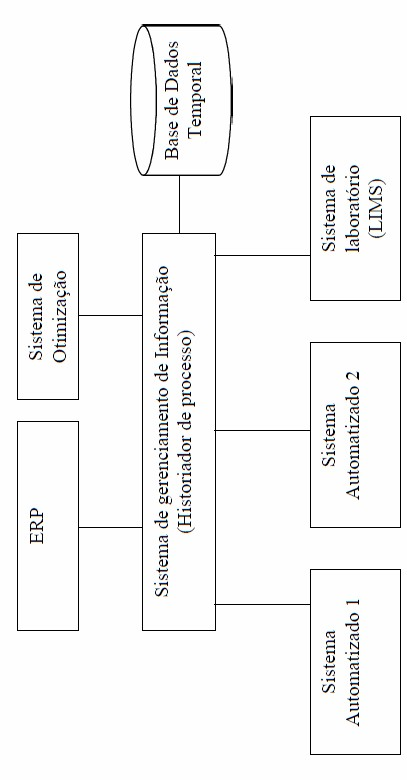
\includegraphics[angle=-90,width=0.8\textwidth]{PIMS}
		\end{center}
		\caption{Sistema PIMS -- REFAZER.}
		\label{fig:PIMS}
	\end{figure}

\subsection{Historiador de Processos}
O historiador do processo é necessário pelas seguintes funcionalidades:
\begin{description}
 	\item[Registro Histórico] para análise de incidentes, controle de qualidade, métricas de performance, entre outros.
 	\item[Adequação a normas] como por exemplo para controle ambiental.
 	\item[Monitoração de equipamentos] para ontrole de vida útil e apoio à manutenção.
 	\item[Análise de processo], facilitando a visualização de dados e detecção de correlações.
 \end{description}  			

Para tanto o historiador se comunica com sistemas do nível 2 (SCADA) e 1 (CLP) para armazenar os dados do processo. Estes dados são principalmente os valores das variáveis do processo, sejam discretos ou contínuos, mas também abarcam outras informações, tais como a ocorrência de alarmes, a marcação de que operador está presente, o período que um equipamento está ligado, entre outros. Cada uma desta isformações é identificada por um marcador único - a chamada \emph{tag}, ao qual também está associado o endereço lógico de onde se obtém tal informação e o tempo em que tal dado foi gerado (\emph{time stamp}). Em alguns casos se associa também uma métrica da qualidade do dado, referente a confiabilidade daquele dado, tal como se o instrumento de medida está calibrado ou não.

Estas informações podem ser obtidas tanto de sistemas SCADA ou de CLPs. Algumas vantagens de pegar informação dos sistemas nível 2 são que: 
\begin{itemize}
	\item o SCADA já converteu os dados para unidades de engenharia enquanto que em alguns CLPs os dados estão em valor bruto (de 0 a 4095);
	\item muitas variáveis são definidas apenas no sistema SCADA, não existindo nos CLPs, tais como o motivo de alarmes ou qual operador está monitorando a operação;
	\item  interface com os sistemas SCADA costuma ser padrão, o que facilita a comunicação e interoperação.
\end{itemize}

Vantagens de obter as informações do CLP são:
\begin{itemize}
	\item busca dos eventos com menor atraso temporal;
	\item pode-se coletar os dados em um ponto único, se todas as redes de CLPs estiverem interligadas;
	\item CLPs são mais confiáveis e apresentam menor suscetibilidade a falhas que os sistemas SCADA.
\end{itemize}

\subsection{Banco de Dados Temporal}
A maioria das análises realizadas nos dados de um sistema PIMS são em função do tempo, logo é comum ele usar um banco de dados que indexa a informação pelo tempo. Basicamente é uma tabela, relacionando \emph{time stamp}, \emph{tag}, tipo de dado (analógico, booleano, texto), valor e qualidade (se houver).

Um problema do uso deste tipo de banco de dados, ao invés dos chamados bancos de dados relacionais, que são bem mais comuns, é que a busca por informação pode ter uma baixa performance quando a quantidade de dados aumenta muito. Esta é a principal razão para que estes sistemas façam uma compressão de dados, que basicamente se resume a não armazenar dados que não tragam muita informação nova. A figura \ref{fig:reconstrucaoDados} mostra a idéia por trás da compressão de dados.

\begin{figure}[hbt]
	\begin{center}
		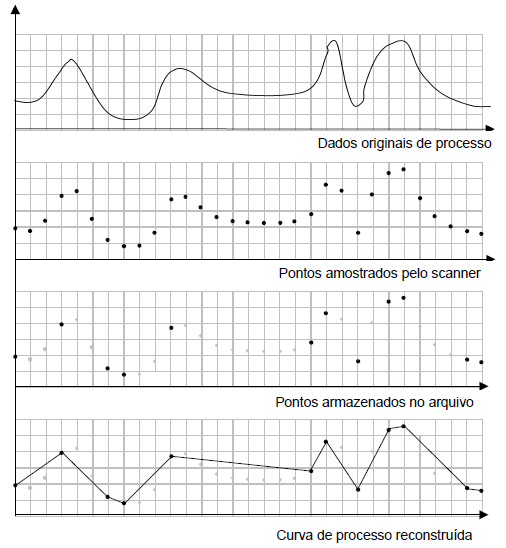
\includegraphics[width=0.8\textwidth]{figuras/reconstrucaoDados}
	\end{center}
	\caption{Processo de amostragem, compressão e reconstrução dos dados.} %%TODO:refazer
	\label{fig:reconstrucaoDados}
\end{figure}

Algoritmos comuns para a compressão de dados no PIMS são \emph{banda morta}, onde os dados são apenas armazenados se variarem mais do que um mínimo especificado; o \emph{SDCA -- Swinging Doors Compression Algorithm}, onde para cada valor recebido é definida uma reta entre ele e o último valor armazenado, descartando valores que possam ser definidos por esta reta e mais um erro; e o \emph{boxcar/backslope}, que usa a banda morta e mais uma reta definida pelo último valor armazenado. %%Pequeno. Pode ser expandido

\subsection{Interface Gráfica}
A interface gráfica de um sistema PIMS é, em muitos aspectos, muito parecida com a de um sistema SCADA, contendo representações pictóricas do processo (sinóticos) com os valores de várias variáveis e gráficos de tendência. Tais elementos são melhor vistos no contexto de um sistema SCADA.

\section{MES}
Assim como o PIMS, um sistema MES também adquire dados do processo com o objetivo de apresentar uma visão geral do processo. Porém o MES tem uma função mais ativa que o PIMS, que é focado mais no armazenamento dos dados. Outra diferença importante é que os MES são usados principalmente em processos discretos, muitas vezes em sistemas de automação flexível ou programada, e tem que lidar com o sequenciamento dos processos, o que ocorre menos em sistemas contínuos.

Os sistemas MES agregam diversas funções de sistemas anteriores mais simples e específicos e são definidos por terem 11 funções:
\begin{description}
	\item[Gerenciamento das definições de produto.] Tudo o que é necessário para a fabricação do produto. Isto inclue armazenamento, lista de materiais e insumos, set-points do processo e receitas.

	Por receita, entenda-se uma variação do processo para, na mesma máquina, produzir produtos diferentes ou variações dele. Por exemplo, num processo de pintura a receita diria quais as tintas usadas, em que sequência, em que volume e em que velocidade de aplicação. É muito importante na automação flexível e programável.

	\item[Gerenciamento de insumos.] Permite preparar e executar ordens de produção com garantia de disponibilidade dos insumos.
	\item[Agendamento de produção.] Permite determinar a ordem que a produção será feita, para alcançar os requerimentos de produção definidos pela ERP (camada 4 da pirâmide) utilizando otimamente os recursos.

	Tipicamente inclui ferramentas de simulação, que permitem comparar diversas opções de ordens e estimar efeitos quando de mudanças imprevistas na sequência de produção (tipicamente por conta de uma parada não programada).

	\item[Envio de ordens de produção.] Em função do agendamento feito, o MES cuida de enviar as ordens de produção para os diversos postos da planta.
	\item[Acompanhamento da execução de ordens de produção.] Comunicação com sistemas níveis 1 e 2 para garantir a execução das ordens. Inclui também o registro de paradas.

	O registro de paradas é feito automaticamente quando o equipamento para, seja por alguma condição espúria detectada no nível 1 ou por ação do operador no nível 2. Em ambos os casos fica registrado uma parada em aberto, que só finaliza quando o operador complementar certas informações que auxiliam no diagnóstico da parada e o equipamento voltar a funcionar.

	\item[Coleção dos dados de produção.] Equivalente ao historiador de processo do PIMS.
	\item[Análise da performance da produção.] Cálculo dos chamados índices de produção -- \emph{KPI, Key Performance Indicators}. É a geração de informação útil a partir dos dados da produção.

	Como exmplo de um KPI, temos o OEE -- \emph{Overall Equipment Effectiveness} -- que aponta a efetividade de um determinado equipamento ou célula de produção. Este índice é dado por:

\begin{equation}
	\text{OEE} = \text{disponibilidade}\times\text{performance}\times\text{qualidade,}
\end{equation}
onde por disponibilidade entende-se a razão entre o quanto de tempo o equipamento funcionou e o quanto de tempo ele deveria ter funcionado, ou seja, descontando-se as paradas não programadas; performance é a razão entre a produção do equipamento enquanto funcionava e a capacidade de produção de que o equipamento é capaz, ou seja, descontando a ociosidade do equipamento; e qualidade é o valor do que o equipamento produziu em relação ao valor se não tivesse havido nenhum descarte ou geração de produtos de menor valor.

	\item[Rastreamento da produção.] Permite levantar que produto ou lote foi feito quando e em qual equipamento. Útil para melhoria da produção e imprescindível para remédios e produtos alimentícios.
	\item[Armazenamento dos logs de produção.] Hoje em dia tais logs são inseridos pelo operador no próprio sistema supervisório e realcionados às variáveis de produção.
	\item[Interface de auditoria.] Permite a análise dos diversos dados e informações armazenados e o cruzamento destes dados com outras bases de dados.
\end{description}